\documentclass[12pt, a4paper, figuresright]{book}
\usepackage{mathtools, commath, amssymb, amsthm}
\usepackage{tabularx,graphicx,url,xcolor,rotating,multicol,epsfig,colortbl,lipsum}
\usepackage[T2A]{fontenc}
\usepackage[english,main=russian]{babel}

\setlength{\textheight}{25.2cm}
\setlength{\textwidth}{16.5cm}
\setlength{\voffset}{-1.6cm}
\setlength{\hoffset}{-0.3cm}
\setlength{\evensidemargin}{-0.3cm} 
\setlength{\oddsidemargin}{0.3cm}
\setlength{\parindent}{0cm} 
\setlength{\parskip}{0.3cm}

\newenvironment{talk}[6]{%
\vskip 0pt\nopagebreak%
\vskip 0pt\nopagebreak%
\textbf{#1}\vspace{3mm}\\\nopagebreak%
\textit{#2}\\\nopagebreak%
#3\\\nopagebreak%
\url{#4}\vspace{3mm}\\\nopagebreak%
\ifthenelse{\equal{#5}{}}{}{Соавторы: #5\vspace{3mm}\\\nopagebreak}%
\ifthenelse{\equal{#6}{}}{}{Секция: #6\quad \vspace{3mm}\\\nopagebreak}%
}

\pagestyle{empty}

\begin{document}
\begin{talk}
{Метод построения ортогональной генерирующей системы узлов разностной сетки для области с криволинейной границей с помощью квазиконформного отображения}
{Возианова Анна Викторовна}
{Университет ИТМО}
{vozianova@itmo.ru}
{Бебех К.\,В.}
{Прикладная математика и математическое моделирование}

Активное развитие проектирования и создания композитных структур со сложной геометрией элементарных ячеек, требует развития и модификации существующих численных методов для учета локальных геометрических особенностей подобных структур. В данной работе предложен метод построения ортогональной генерирующей системы узлов разностной сетки для области с искривленной границей.

В ортогональной сетке все недиагональные элементы метрического тензора g равны нулю:
\begin{align*}
g_{ij} = \frac{\partial x}{\partial \xi} \frac{\partial x}{\partial \eta}+\frac{\partial y}{\partial \eta} \frac{\partial y}{\partial \xi} = 0,~ i\ne j,~ \sqrt{det g} = \sqrt{g_{11}g_{22}} = h_{xi}h_{\eta}   
\end{align*}
где \(g_{11},~g_{22}\) - коэффициенты метрического тензора, \(h_{xi},~h_{\eta}\) - коэффициенты Ламе.
Двумерная ортогональная сетка должна удовлетворять уравнениям Бельтрами:
\begin{align*}
f \frac{\partial x} {\partial \xi} =\frac{\partial y}{\partial \eta},~f \frac{\partial y}{\partial \eta} = -\frac{\partial x}{\partial \xi} 
\end{align*}
где \(f= \frac{h_{xi}}{h_{\eta}}\) - функция искажения.
Мощным аппаратом для нахождения материальных параметров структуры с помощью метрического тензора и геометрии среды является новая наука о манипуляции излучением --– трансформационная оптика [1].
\medskip
\begin{figure}[h!]
\centering
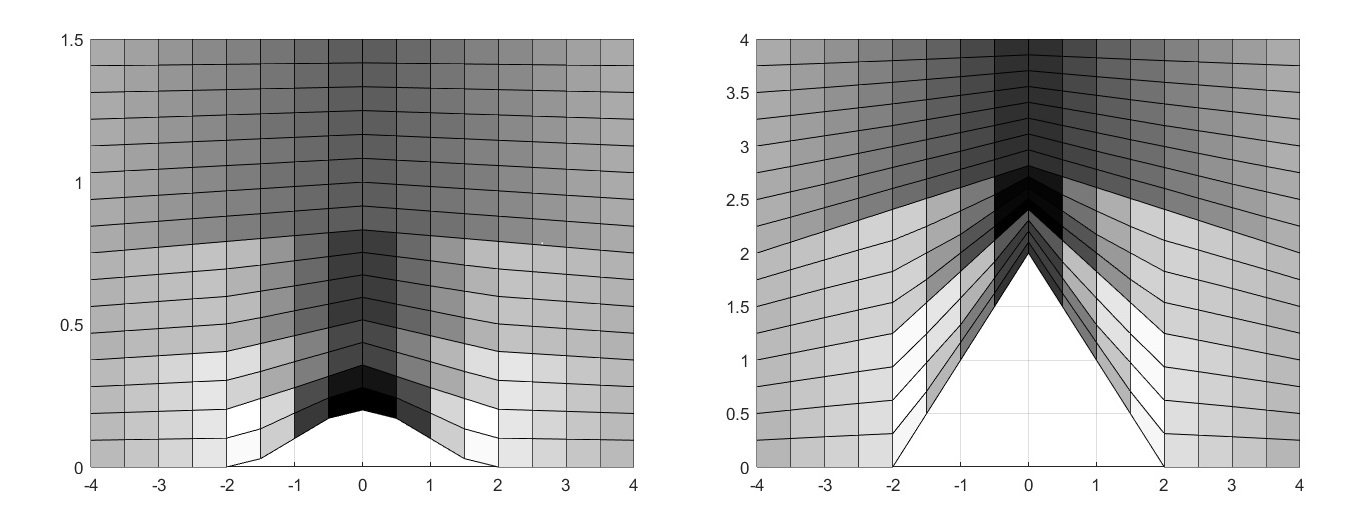
\includegraphics[width=0.75\linewidth]{Возианова.jpeg}
\caption{Разностная сетка и распределение показателя преломлнения в анизотропном материале (a) произвольное искажение границы, (b) линейное искажение границы.}
\label{fig:dist}
\end{figure}
Предложенный метод аппробирован на проектировании анизотропного материала с различным показателем преломления в каждой ячейке, как показано на рисунке. 
\begin{enumerate}
\item[{[1]}] UlfLeonhardt, Tomas Philbin , {\it Geometry and light: the science of invisibility},  Mineola, New-York: Dover Publication, Inc., 2010.
\end{enumerate}
\end{talk}
\end{document}
